\subsection{SD-Karte}
\label{subsec:SD-Karte}

Damit gespeicherte Getränke, Zutaten und Maschinenzustände bei einem Neustart der Cocktailmaschine erhalten bleiben, werden diese auf der SD-Karte abgelegt. Nebst dem Erhalten der Informationen ist die SD-Karte wichtig für den Betrieb der Maschine. Werden zu viel Getränke und Zutaten auf dem Mikrocontroller gespeichert, so führt dies zu einem Absturz des Mikrocontrollers. Es wurde daher entschieden, eine mikroSD-Karte zu verwenden. Im Folgenden wird erklärt, was es Hard- und Softwaretechnisch zu beachten gab.

Abbildung \ref{fig:micro_sd_pinout} zeigt die Pinbelegung einer mikroSD-Karte. Es ist erkennbar, dass sie über SPI kommuniziert. Für den Anschluss wird nur ein mikroSD-Sockel benötigt. So kann die mikroSD über einen Level-Shifter vom Mikrocontroller angesteuert werden. Der Level-Shifter wird verwendet, da der Mikrocontroller mit 5V-Signalen arbeitet und die SD-Karte mit 3,3V arbeitet.

\begin{figure}[H]
	\centering
	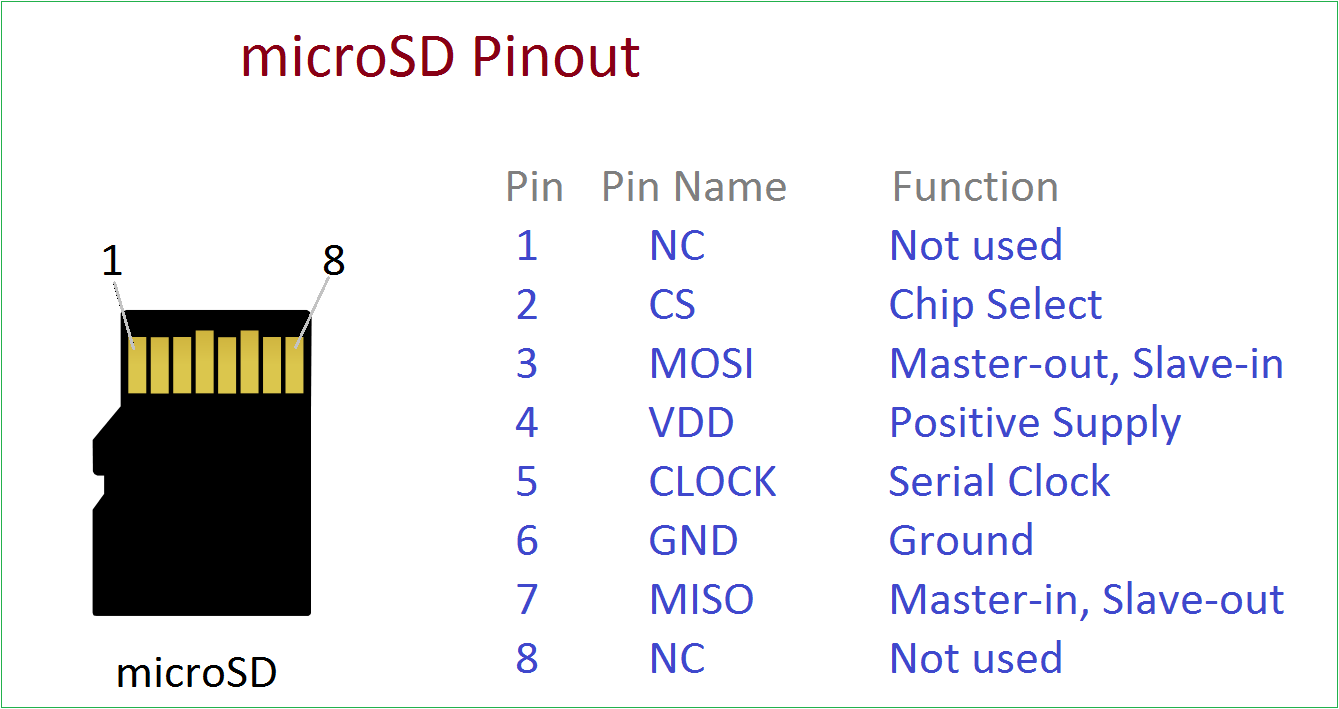
\includegraphics[width=0.55\textwidth]{graphics/micro-sd-pinout}
	\caption{Pinout des mikroSD-Sockels. \cite{theorycircuitcom_arduino_2018}}
	\label{fig:micro_sd_pinout}
\end{figure}

Als Dateisystem wird FAT32 verwendet. FAT32 steht für File Allocation Table mit 32Bit Datenbreite. Es ist ein von Micosoft entwickeltes System, dessen Wurzeln bis ins Jahr 1977 zurückreichen und heute noch der Industriestandard unter den Dateisystemen ist. \cite{ionosde_fat32_2020}

Der Speicherbereich einer FAT32-formatierten Partition besteht aus fünf Bereichen. \cite{milsch_aufbau_2009}
\begin{enumerate}
\item Master Boot Record (LBA Sektor 0 des Laufwerks)
\item Volume Boot Record, Partition Boot Sektor (LBA Sektor 0 der Partition)
\item File Allocation Table (i.d.R 2 mal hintereinander vorhanden, direkt nach dem PBR)
\item Directory Table (mit den Ordner und File-Einträgen)
\item Datenbereich (Fileinhalt)
\end{enumerate}

Im Anhang Kapitel \ref{Appendix:FAT32_Aufbau} sind die einzelnen Bereiche detailliert beschrieben.

Für den PartyMixer wird softwareseitig eine Library benötigt, welche die FAT32-Commands  implementiert und gleichzeitig die Operationen auf der SD-Karte abhandelt. So ist die SD-Karte auch am Computer editierbar und die Befehlsliste reduziert sich auf readFile, writeFile und deleteFile.

\paragraph{Schema}\mbox{}

In Abbildung \ref{fig:Schema_SD_Karte} ist das Schema der SD-Karte zu sehen. Darin erkennbar ist der mikroSD-Adapter J45 mit einem Stützkondensator C68 am Spannungseingang.

\begin{figure}[H]
\center
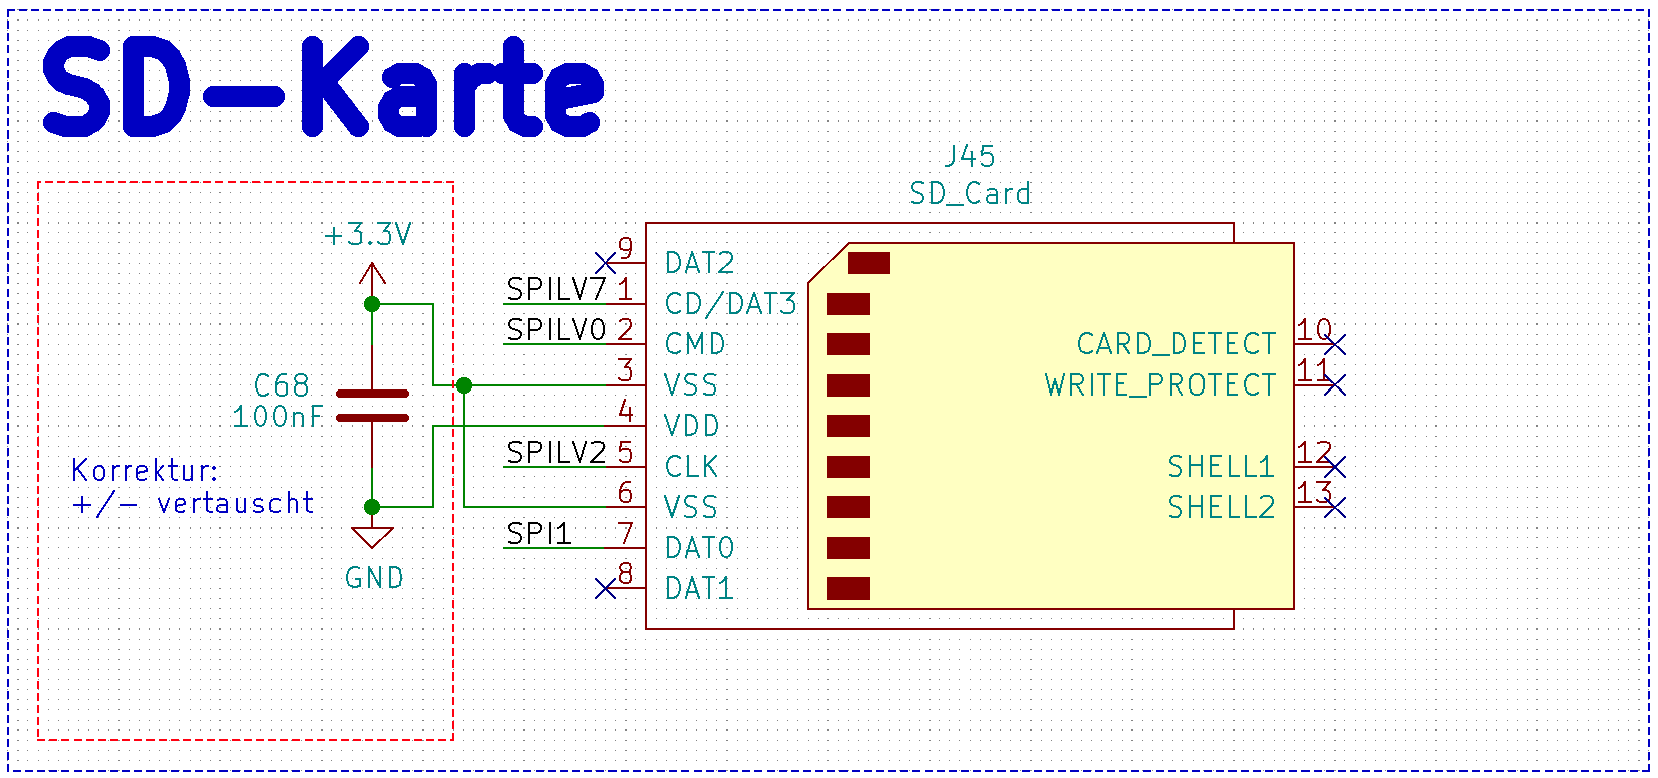
\includegraphics[width = 0.6 \textwidth]{graphics/Schema_SD_Karte}
\caption{Schema SD-Karte.}
\label{fig:Schema_SD_Karte}
\end{figure}

\paragraph{Funktionsbeschrieb der Schaltung}\mbox{}

In der Schaltung ist erkennbar, dass die SPI-Leitungen an die Pins des Adapters führen, genauso die Spannungsleitungen. Da die SD-Karte stets vom Mikrocontroller angesteuert wird, gibt es keine weiteren erwähnenswerte Funktionen zu beschreiben.